\chapter{Métodos Estadísticos Para Procesamiento de Datos}
\label{ch:Estadisticos}

\section{Conceptos Básicos}

La Estadística es una disciplina derivada de las Matemáticas que puede definirse de diferentes formas según el autor y su área de aplicación. En \cite{triola} se define la Estadística como una colección de métodos para planear 
experimentos, obtener datos, y después organizar, resumir, presentar, analizar, interpretar, y llegar a conclusiones basadas en los datos.    

En \cite{anderson} la Estadística se define como el arte y la ciencia de reunir datos, analizarlos e interpretarlos, lo cual permite mejorar la toma de decisiones en la aplicación específica donde estos métodos sean aplicables.

En las 2 definiciones anteriores hay un concepto que se repite, el de datos; ambas definiciones están construidas en torno a la palabra datos. Por lo tanto, desde aquí se puede apreciar que la Estadística se fundamenta y 
entrega resultados partiendo de datos o información que es buscada en el entorno de trabajo donde se desea aplicar la Estadística para la obtención de conclusiones.

En \cite{anderson} Datos se definen como hechos/informaciones y cifras numéricas que se recogen, analizan y resumen para su presentación e interpretación. 

\clearpage

\section{Tipos de Datos}

La \autoref{fig:figura600_1} muestra el diagrama de los tipos de datos usados en Estadística.

\begin{figure}[h]
	\centering
	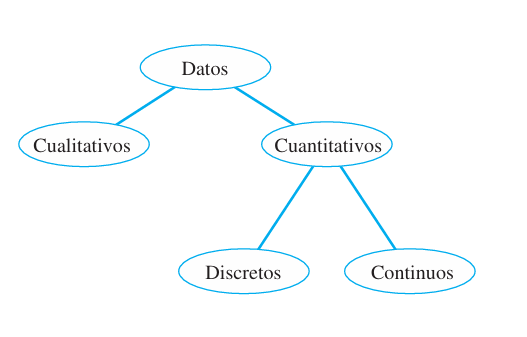
\includegraphics[scale=0.7]{imgss140.png}
	\caption{Tipos de datos}
	\label{fig:figura600_1}
\end{figure}

Los datos cualitativos son aquellos formados por etiquetas o nombres que permiten identificar un atributo de un objeto o persona \cite{anderson}. A los datos cualitativos también se les suele llamar datos categóricos o datos 
de atributo. Un ejemplo de este tipo de datos sería el color de una prenda de vestir, es decir, el dato \textit{color} podría tomar valores tales como azul, rojo, negro, verde, morado, entre otros.

Los datos cuantitativos son aquellos que consisten en números que representan conteos o mediciones \cite{triola}. Los datos cuantitativos pueden dividirse en 2 categorías, datos discretos y datos continuos.

Los datos discretos son aquellos que resultan cuando el número de posibles valores es un número finito, o bien, un número que puede contarse \cite{triola}. Un ejemplo de datos discretos sería la cantidad de personas presentes 
en un lugar específico.

Los datos continuos resultan de un número infinito de posibles valores que se pueden asociar a puntos de una escala continua, cubriendo un rango de valores sin huecos ni interrupciones \cite{triola}. Un ejemplo sería los 
valores de magnitud de la velocidad a la cual se desplaza un vehículo.

\section{Fuentes de Obtención de los Datos}

Se reconocen 2 métodos para la recolección de nuevos datos.

\begin{itemize}
    \item \textbf{Fuentes existentes}. Es posible que para una aplicación específica los datos requeridos ya existan. Por ejemplo, los sitios de internet gubernamentales contienen miles de bases de datos sobre diversas temáticas,
	y en su mayoría son de acceso libre con excepción de bases de datos que contengan datos confidenciales o información personal \cite{anderson}. 
    \item \textbf{Estudios estadísticos}. Es la metodología implementada cuando los datos no existen y deben obtenerse. Existen 2 tipos de estudios estadísticos, los experimentales y los observacionales. En la realización de un 
    estudio experimental primero se debe establecer cuál es la variable de interés, y después definir 1 o más variables de control, las cuales son modificadas para obtener información de cómo afectan a la variable de interés.
	Por otro lado, un estudio observacional consiste básicamente en la realización de una encuesta, por ejemplo, salir a realizar preguntar a un número definido de personas acerca del tema que se está estudiando \cite{anderson}. 
\end{itemize}

\clearpage

Adicionalmente, deben definirse 2 conceptos básicos relacionados con la recolección de datos en estadística.

\begin{itemize}
    \item \textbf{Variable}. Característica que cambia o varía con el tiempo para diferentes personas, objetos o entornos \cite{mendenhall}.
    \item \textbf{Unidad experimental}. Es el individuo, objeto o entorno en el que se mide una variable \cite{mendenhall}. 
    \item \textbf{Medición}. Dato obtenido para una variable \cite{mendenhall}.
    \item \textbf{Población}. Conjunto de mediciones de interés \cite{mendenhall}.
    \item \textbf{Muestra}. Subconjunto de mediciones obtenido de la Población \cite{mendenhall}.
\end{itemize}

\section{Estadística Descriptiva}

La estadística descriptiva consiste en la presentación o exposición de los datos recolectados, a través del uso de resúmenes, los cuales pueden ser tabulares, gráficos o numéricos \cite{anderson}.

Para nuestros propositos, los resúmenes de tipo numérico serán los de mayor utilidad acorde a las características del proyecto realizado.

\begin{itemize}
    \item \textbf{Media o Promedio}. El valor promedio de una variable proporciona una medida de localización central de los datos de una variable. Su cálculo tiene la forma (\ref{eq:ecuacion601}).
    \begin{equation}
	\mu=\frac{\sum_{i=0}^{N} {(x_i)}}{N}
	\label{eq:ecuacion601}
    \end{equation}

	Es decir, el valor promedio de un conjunto de datos es igual a la sumatoria de todos los datos, dividida entre el número de datos.

    \item \textbf{Mediana}. Para un conjunto de datos, la mediana es el valor de enmedio para dichos datos ordenados de menor a mayor, es decir, en forma ascendente \cite{anderson}. 
    
	Si el número de datos es impar, la mediana es el valor de enmedio. Si el número de datos es par, la mediana es el promedio de las 2 observaciones de enmedio \cite{anderson}. Si el número de datos es par, se puede usar 
	la ecuación (\ref{eq:ecuacion6058}) para obtener la mediana.
    
	\begin{equation}
	MED(X)=\frac{X(n/2) + X(1 + n/2)}{2}
	\label{eq:ecuacion6058}
    \end{equation}

	Es decir, la mediana de un conjunto de datos \textit{X} par se obtiene al sacar el promedio de los datos en las posiciones \textit{n/2} y \textit{1 + n/2} del arreglo de datos.

	\item \textbf{Moda}.La moda de un conjunto de datos es el valor que se repite con mayor frecuencia \cite{anderson}.
	\item \textbf{Rango}. El rango para un conjunto de datos es igual a la diferencia del valor mayor del conjunto y el valor menor \cite{anderson}.
	
	\begin{equation}
		Rango=Valor Mayor - Valor Menor
		\label{eq:ecuacion602}
	\end{equation}

	\item \textbf{Varianza}. La varianza de un conjunto de datos es una medida de su variabilidad, la cual se basa en la diferencia entre el valor de cada dato y el promedio de los datos; a dicha diferencia se le suele denominar \textit{desviación respecto a la media} \cite{anderson}.
	
	Si la varianza se calcula para los datos de una Población, se le conoce como \textit{varianza poblacional}, y se calcula de la forma (\ref{eq:ecuacion603})

	\begin{equation}
		\sigma^2=\frac{\Sigma (x_i - \mu)^2 }{N}
		\label{eq:ecuacion603}
	\end{equation}

	Si la varianza se calcula para datos que provienen de una muestra, se le dennomina \textit{varianza muestral} y se calcula de la forma (\ref{eq:ecuacion604})

	\begin{equation}
		s^2=\frac{\Sigma (x_i - \mu)^2 }{N-1}
		\label{eq:ecuacion604}
	\end{equation}

	A la varianza muestral se le considera el mejor estimador de la varianza poblacional para casos en donde no es posible el cálculo de la varianza poblacional debido principalmente a que no se conoce a toda la Población \cite{anderson}.

	\item \textbf{Desviación Estándar}. Se define como la raíz cuadrada positiva de la varianza \cite{anderson}. Al igual que para la varianza, para la desviación estándar existen la \textit{desviación estándar poblacional} (\ref{eq:ecuacion605})
	
	\begin{equation}
		\sigma=\sqrt{\sigma^2}
		\label{eq:ecuacion605}
	\end{equation}

	y la \textit{desviación estándar muestral} (\ref{eq:ecuacion606})

	\begin{equation}
		s=\sqrt{s^2}
		\label{eq:ecuacion606}
	\end{equation}

	De nuevo la desviación muestral es el mejor estimador de la desviación poblacional cuando su cálculo no es posible.

\end{itemize}

\subsection{Datos Atípicos}

Cuando se realiza la recolección de datos en una aplicación dada, y al analizarlos se detectan datos cuyos valores son mucho más grandes o mucho más pequeños que la mayoría de los datos recolectados, a estos valores extremos 
se les conoce como \textit{datos atípicos} u \textit{observaciones atípicas} \cite{anderson}.

Cuando se detectan este tipo de casos, es importante actuar con precaución acerca de cuál es la razón de tener datos atípicos. Es decir, puede que la causa sea que el investigador cometió un error al escribir el valor de 
un dato, algún error en la metodología o equipo de medición, pero también puede ser el caso de que el dato atípico realmente sí pertenezca al conjunto de datos, es decir, que no existe error en su recolección, por lo tanto, 
ese comportamiento inusual en los valores de los datos también deberá considerarse como parte del conjunto de datos \cite{anderson}.

\section{Coeficiente de Correlación Lineal de Pearson}

En estadística descriptiva al tener aplicaciones en las cuales en la mayoría de ellas se recolectan datos de una gran cantidad de variables, es conveniente realizar un análisis matemático acerca de si existen posibles 
relaciones entre algunas de estas variables. Pero, ¿qué tipo de relación entre ellas es útil buscar? Principalmente, el concepto de este análisis es tomar una variable como pivote, y ver qué ocurre con los datos de las 
demas variables cuando los datos de la variable pivote aumentan o decrecen en su magnitud de valor numérico. Por ejemplo, teniendo una variable pivote y una variable de prueba para análisis, se puede estudiar el comportamiento
de los datos de la variable de prueba cuando los datos de la variable pivote crecen o decrecen \cite{pinilla_pearson_2021}.

Primeramente, consideremos la \autoref{fig:figura600_2} 

\begin{figure}[h]
	\centering
	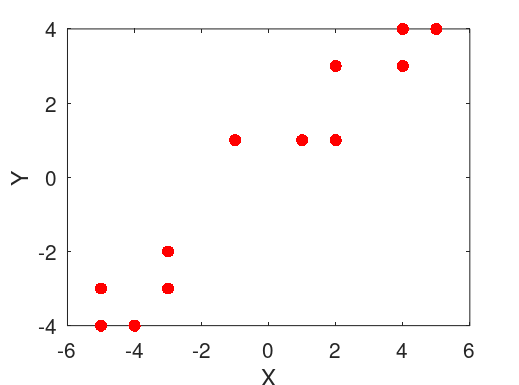
\includegraphics[scale=0.7]{imgss141.png}
	\caption{Relación lineal positiva entre 2 variables}
	\label{fig:figura600_2}
\end{figure}

En la \autoref{fig:figura600_2} podemos ver graficados los datos de 2 variables, "X vs Y". Se pueden establecer 2 conclusiones sobre los datos de dichas variables. La primera conclusión sería que de forma general el comportamiento 
entre dichas variables obedece a que cuando la variable X crece, la variable Y igualmente incrementa su valor. La segunda conclusión es sobre el hecho de que podríamos trazar una recta diagonal en la gráfica y dicha recta 
pareciera que sigue la tendencia marcada por los puntos. A partir de estas 2 conclusiones, podemos definir este comportamiento como una \textit{relación lineal positiva} entre las 2 variables contrastadas.

Ahora se considera la \autoref{fig:figura600_3}

\begin{figure}[h]
	\centering
	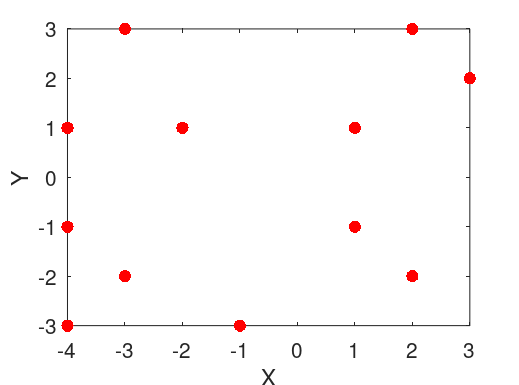
\includegraphics[scale=0.7]{imgss142.png}
	\caption{No existe relación lineal entre las variables}
	\label{fig:figura600_3}
\end{figure}

Igualmente, en la \autoref{fig:figura600_3} volvemos a tener un contraste de 2 variables "X vs Y". En este segundo caso, no se puede establecer que un incremento en la variable X esté correspondido con un incremento en 
la variable Y. De la misma forma, no se logra definir que una recta logre replicar el comportamiento de los datos marcados en la gráfica. Por lo tanto, para este segundo caso no existe ningún tipo de relación lineal.

Finalmente, consideremos la \autoref{fig:figura600_4}

\clearpage

\begin{figure}[h]
	\centering
	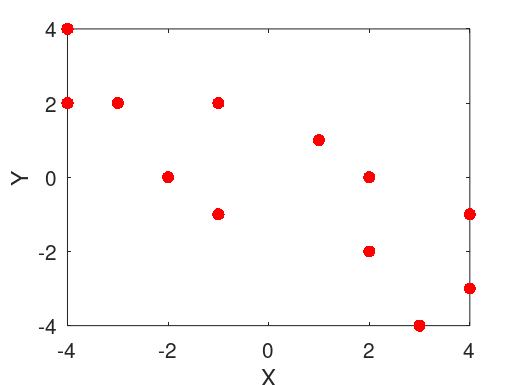
\includegraphics[scale=0.7]{imgss143.png}
	\caption{Relación lineal negativa entre 2 variables}
	\label{fig:figura600_4}
\end{figure}

Volvemos a tener un contraste entre variables "X vs Y". Para este tercer y último caso se puede observar una tendencia inversa entre las variables, es decir, cuando la variable X incrementa su valor, el comportamiento 
de la variable Y tiende a ser decreciente. Para este tipo de gráfica si trazamos de nuevo una recta en diagonal, ésta podra ayudarnos nuevamente a replicar la tendencia marcada por los datos, aunque en este tercer caso 
la recta tendrá una pendiente negativa. A este tipo de comportamiento entre 2 variables, se le denomina \textit{relación lineal negativa o inversa}.

Ahora que se sabe que pueden existir diferentes tipos de relación entre distintas variables, el objetivo en esta sección es cuantificar esa relación, es decir, obtener una medida numérica que pueda indicar el tipo de 
relación en caso de que exista, así como poder conocer la \textit{fuerza} de la relación entre 2 variables \cite{anderson}. Para esto se cuenta con la herramienta matemática del \textit{coeficiente de correlación de Pearson} (\ref{eq:ecuacion607})

\begin{equation}
	%r=\frac{\frac{\Sigma (x_i - \mu_x)(y_i - \mu_y) }{N}}{\sigma_x \sigma_y}
	r=\frac{1}{\sigma_x \sigma_y} \frac{\sum_{i=0}^{N} (x_i - \mu_x)(y_i - \mu_y)}{N}
	\label{eq:ecuacion607}
\end{equation}

Es decir, el cálculo de este indicador implica la sumatoria de los productos de las diferencias de los datos y sus promedios correspondientes, así como dividir estos resultados entre el producto de las desviaciones estándar
de cada una de las variables que se están comparando.

El rango de valores que puede tomar el coeficiente de Pearson abarca desde -1 hasta +1. Si el cálculo del coeficiente de Pearson entrega un resultado de +1, esto implica que los datos analizados se encuentran sobre una 
línea recta con pendiente positiva, conociéndose esto como una \textit{relación lineal positiva perfecta}. Por el contrario, si el cálculo del coeficiente entrega un resultado de -1, esto significa que los datos se encuentran 
sobre una línea recta con pendiente negativa, y a este caso se le conoce como \textit{relación lineal negativa perfecta} entre las 2 variables analizadas \cite{anderson}.

Si los datos de las variables comparadas muestran una relación lineal positiva, pero no es perfecta, esto implica que el valor del coeficiente sera menor a 1, indicando que no todos los puntos de la gráfica de los datos se 
encuentran sobre una línea recta. Entre más se desvién los puntos de una línea recta, menor sera el valor del coeficiente de correlación. Si el valor del coeficiente de correlación entrega un resultado de 0, significa que no 
existe una relación lineal entre las 2 variables analizadas; si el valor del coeficiente no es 0 pero cercano a dicho valor, significa que la relación lineal entre las 2 variables es \textit{débil} \cite{anderson}.

Finalmente, en este tema hay que dejar claro que el coeficiente de Pearson es un indicador de la medida de la relación lineal de 2 variables, mas no un indicador de causalidad. Es decir, si la correlación lineal entre 2 
parámetros es alta, esto no significa que los cambios que presente una de las variables, implique o genere cambios en la otra variable \cite{anderson} \cite{mendivelso_prueba_2022}.

\section{Conclusiones}

La estadística descriptiva tiene como objetivo tomar un conjunto de datos y realizar una caracterización de estos que permita conocer qué tipo de datos se tienen y el tipo de comportamiento que presentan. Para el trabajo 
desarrollado en esta tesis se ejecutan un cierto número de muestreos de agua en un proceso de potabilización, y dichas muestras serán analizadas para diferentes parámetros de calidad recolectando una gran cantidad de datos 
para cada una de las variables en estudio. Por lo tanto, la estadística descriptiva se convierte en la herramienta más útil para poder generar un panorama completo de las características que poseen los datos recolectados, 
lo que a su vez nos permite entender gran parte del comportamiento de la calidad del agua durante las diferentes etapas del proceso de potabilización.

Por otra parte, la herramienta del coeficiente de correlación lineal nos permite conocer si los diferentes parámetros de calidad del agua estudiados presentan entre ellos un patrón de comportamiento específico que nos permita 
establecer que dichas variables tienen ese patrón o tendencia debido a los cambios dados por el proceso de tratamiento. Además, el tener un nivel de correlación alto entre diferentes parámetros nos permite conocer el comportamiento 
de otras variables si se conoce el comportamiento de un parámetro específico. 

Todas las conclusiones y resultados que se pueden obtener de la aplicación de métodos estadísticos son la referencia principal que se puede seguir para la elección de las variables de calidad del agua que serán utilizadas 
como parámetros de entrenamiento en el modelo de red neuronal para clasificación de calidad del agua.
